\chapter{Methadology}

\section{Data Collection}
The data collection process for this methodology involves several intricate steps, leveraging multiple data sources and employing various Python-based techniques 
to gather and process the required information. This section outlines the comprehensive approach taken to ensure the data is robust, reliable, and suitable for subsequent analysis and modeling.

\subsection{Financial Market Data Acquisition}
The first step in the data collection process involves obtaining financial market data from Yahoo Finance. This includes historical prices and volumes for a range of 
assets such as Bitcoin (BTC), Ethereum (ETH), Solana (SOL), gold, oil, Nvidia, the VIX, S\&P 500, and Dow Jones Industrial Average. The Python yfinance library is employed 
to access the Yahoo Finance API. This library provides an efficient way to retrieve historical price data, allowing us to gather data spanning the past five years. 
The collected data includes:

\begin{itemize}
    \item Daily closing prices
    \item Trading volumes
\end{itemize}

This data forms the foundation of the dataset, providing crucial information on market trends and volatility.

\subsection{Google Trends and Wikipedia Data}
To gauge public interest and sentiment, data from Google Trends and Wikipedia is incorporated. For Google Trends, the focus is on terms such 
as 'bitcoin', 'ethereum', 'solana', 'crypto', and 'blockchain'. This data is accessed using the pytrends library, which allows us to download historical 
search interest data for these terms. Similarly, Wikipedia page views for the same terms are collected using the Wikipedia API. The aggregation of this data
 involves summing the total page views and total search interest over the specified period. This provides a measure of the general public's engagement and interest in these topics.

\subsection{Reddit Sentiment Analysis}
Sentiment analysis is performed on Reddit posts related to Solana, sourced from three specific subreddits. The data is pulled using the Reddit API, focusing on the top 100 posts 
at the time of collection. The information retrieved includes:

\begin{itemize}
    \item Post titles
    \item Post descriptions (selftext)
    \item Number of upvotes
    \item Date posted
\end{itemize}

A sentiment analysis pipeline is implemented using the VADER (Valence Aware Dictionary and sEntiment Reasoner) sentiment analysis tool. The text data is 
preprocessed to remove noise, and sentiment scores are computed for each post. These scores are then aggregated by date, weighted by the number of upvotes, 
to calculate a mean weighted average sentiment for each day. This approach ensures that posts with higher engagement have a more significant impact on the sentiment measure.

\subsection{Total Value Locked (TVL)}
The total value locked (TVL) data for each cryptocurrency is obtained from Defi Lama. TVL represents the total capital held within a blockchain's DeFi ecosystem, 
providing insight into the level of trust and engagement from the community. This data is crucial for understanding the financial health and adoption of each cryptocurrency.

\subsection{Technical Indicators}
Technical indicators are derived from the historical price data obtained in the first step. A Python function is developed to calculate several key indicators, including:

\begin{itemize}
    \item Moving Average (MA)
    \item Exponential Moving Average (EMA)
    \item Stochastic Oscillators
    \item Relative Strength Index (RSI)
    \item Commodity Channel Index (CCI)
    \item Moving Average Convergence Divergence (MACD)
\end{itemize}

These indicators are used to create trend deterministic columns, where a value of 1 indicates a bullish signal and 0 indicates a bearish signal. 
These technical indicators are essential for understanding market trends and potential future movements.

\subsection{Data Merging and Preparation}
The final step in the data collection process involves merging all the collected data on the date field. This step integrates the financial market data, Google Trends and Wikipedia data,
 Reddit sentiment scores, TVL data, and technical indicators into a single cohesive dataset. The merged dataset is then ready for feature selection and modeling, ensuring that all relevant 
 information is available for comprehensive analysis.




\section{Feature Engineering}

\subsection{Technical Indicators:} Calculation of moving averages, RSI, MACD, Bollinger Bands, etc., using historical price and volume data.
\subsection{Reddit Sentiment Analysis:} Top 100 posts from Reddit communities for Bitcoin, Ethereum, and Solana. Sentiment analysis using VADER lexicon to derive bullish or bearish sentiment scores.
\subsection{Additional Features:} Inclusion of market indices data (S\&P 500, NVIDIA) as predictors.


\section{Machine Learning Models}
\subsection{Random Forest}
Random Forest is an ensemble learning method that operates by constructing a multitude of decision trees during training and outputting the mode of the classes (classification) or mean prediction (regression) of the individual trees. The principle behind Random Forest is to reduce the risk of overfitting by averaging multiple deep decision trees, trained on different parts of the same training set.

Mathematically, for a given input $\mathbf{x}$, the prediction of the $i$-th tree $h_i(\mathbf{x})$ in a random forest is:
\[
f(\mathbf{x}) = \frac{1}{N} \sum_{i=1}^N h_i(\mathbf{x})
\]
where $N$ is the number of trees in the forest.

Key parameters include:
\begin{itemize}
    \item Number of trees ($N$)
    \item Maximum depth of each tree
\end{itemize}

\subsection{Support Vector Classification (SVC)}

Support Vector Classification (SVC) aims to find the optimal hyperplane that maximizes the margin between the classes. This hyperplane is defined by the support vectors, which are the data points closest to the hyperplane.

The optimization problem for SVC can be written as:
\[
\min_{\mathbf{w}, b} \frac{1}{2} \|\mathbf{w}\|^2 \quad \text{subject to} \quad y_i (\mathbf{w} \cdot \mathbf{x}_i + b) \geq 1, \; \forall i
\]
where $\mathbf{w}$ is the weight vector, $b$ is the bias, $\mathbf{x}_i$ are the input vectors, and $y_i$ are the class labels.

Key parameters include:
\begin{itemize}
    \item Kernel type (linear, polynomial, radial basis function)
    \item Regularization parameter ($C$)
\end{itemize}

\subsection{Gradient Boosting Classification}

Gradient Boosting Classification is a sequential ensemble technique that builds models in a stage-wise manner. It optimizes for a loss function by adding weak learners to the model, typically decision trees.

The prediction function is of the form:
\[
F_m(\mathbf{x}) = F_{m-1}(\mathbf{x}) + \eta h_m(\mathbf{x})
\]
where $F_m$ is the prediction at stage $m$, $\eta$ is the learning rate, and $h_m$ is the weak learner added at stage $m$.

Key parameters include:
\begin{itemize}
    \item Learning rate ($\eta$)
    \item Number of estimators
    \item Maximum depth of each estimator
\end{itemize}

\subsection{Long Short-Term Memory (LSTM)}

Neural networks often seem like black boxes: inputs go in, outputs come out, and decisions rely on current inputs. However, neural networks do have memory in their learned weights, 
which reflect training data, though this memory is static. Some scenarios, like stock market analysis, require remembering inputs over time for better decisions.

To handle time series data, neural networks can be connected to process each time step individually, feeding data within a context window to capture the necessary information. 
Periodic patterns, like predicting annual Christmas tree sales, need either a large context window or a memory system that retains valuable data and discards the irrelevant.

Recurrent neural networks (RNNs) theoretically address this but suffer from vanishing and exploding gradients, making them impractical. 
Long Short-Term Memory (LSTM) networks solve this by introducing a memory unit called the cell, effectively managing temporal data. 
This diagram shows an LSTM building block.

\begin{figure}[h]
    \centering
    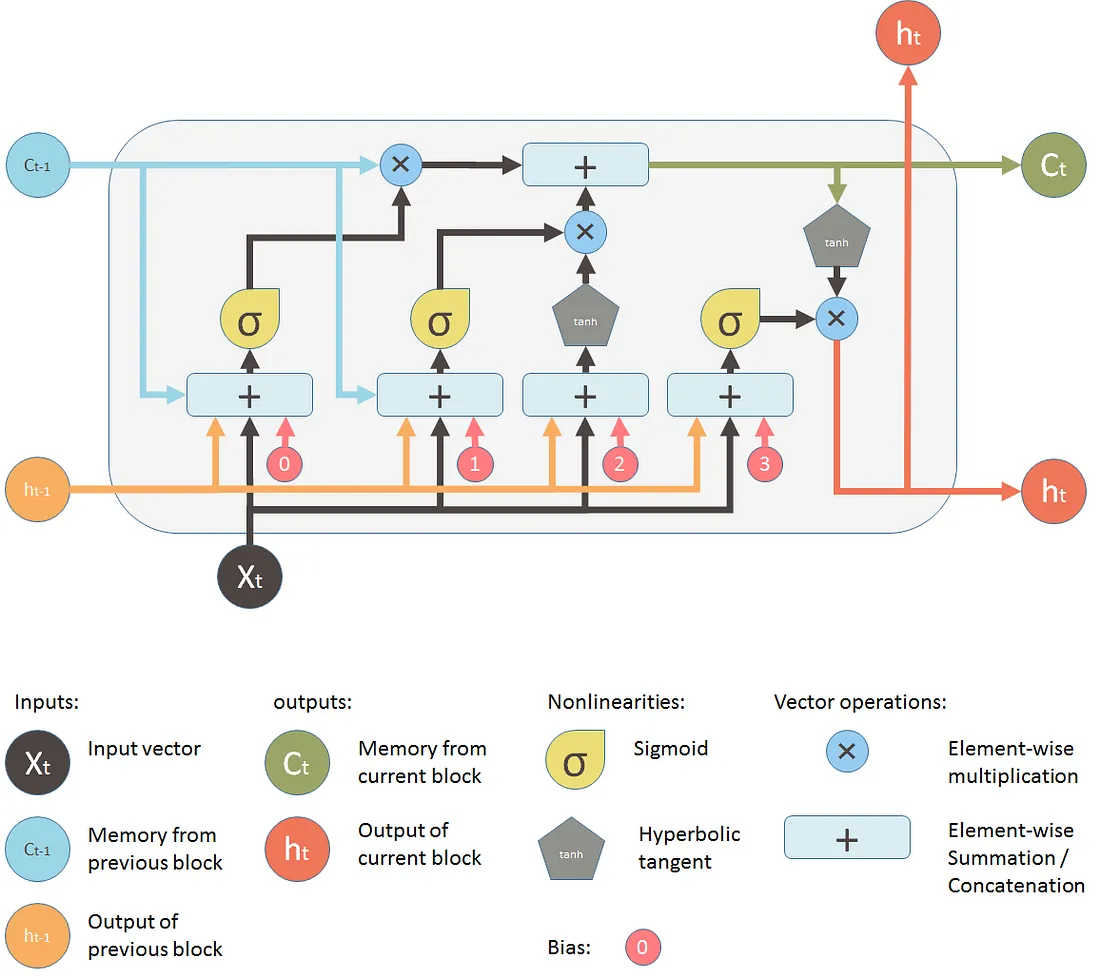
\includegraphics[width=\textwidth]{lstm.png}
    \caption{Caption for the image}
    \label{fig:example-image}
\end{figure}



\subsection{Hidden Markov Model (HMM)}

Hidden Markov Models (HMMs) are statistical models used for sequential data, where the system being modeled is assumed to be a Markov process with hidden states.

An HMM is defined by:
\begin{itemize}
    \item Number of hidden states ($N$)
    \item Transition probability matrix $A = \{a_{ij}\}$, where $a_{ij} = P(s_{t+1}=j | s_t=i)$
    \item Emission probability matrix $B = \{b_j(o_t)\}$, where $b_j(o_t) = P(o_t | s_t=j)$
\end{itemize}

The model works by estimating the sequence of hidden states given the observed data, typically using algorithms such as the Forward-Backward algorithm or Viterbi algorithm.

\[
P(O | \lambda) = \sum_{all \; paths} P(O, Q | \lambda)
\]

where $O$ is the sequence of observations, $Q$ is the sequence of hidden states, and $\lambda = (A, B, \pi)$ represents the model parameters.

An illustrative image showing the state transitions and observation emissions would help explain HMMs more effectively.


\section{Model Evaluation}
\begin{itemize}
    \item \textbf{Metrics:} Accuracy, precision, recall, F1-score, ROC-AUC for classification; MSE, MAE, R-squared for regression.
    \item \textbf{Cross-Validation:} K-fold cross-validation.
    \item \textbf{Model Comparison:} Performance metrics comparison to select the best model.
\end{itemize}
